\chapter{Python Lists}

Watch CS Dojo's \textbf{Introduction to Lists in Python} video at \url{https://www.youtube.com/watch?v=tw7ror9x32s}

To review, Python list is an indexed collection. The indices start at
zero. You can create a list using square brackets.

Now you are going to write a program that makes an array of
strings. Type this code into a file called \url{faves.py}:

\begin{Verbatim}
favorites = ["Raindrops", "Whiskers", "Kettles", "Mittens"]
favorites.append("Packages")
print("Here are all my favorites:", favorites)
print("My most favorite thing is", favorites[0])
print("My second most favorite is", favorites[1])
number_of_faves = len(favorites)
print("Number of things I like:", number_of_faves)

for i in range(number_of_faves):
    print(i, ": I like", favorites[i])
\end{Verbatim}

Run it:
\begin{Verbatim}[commandchars=\\\{\}]
$ \textbf{python3 faves.py}
Here are all my favorites: ['Raindrops', 'Whiskers', 'Kettles', 'Mittens', 'Packages']
My most favorite thing is Raindrops
My second most favorite is Whiskers
Number of things I like: 5
0 : I like Raindrops
1 : I like Whiskers
2 : I like Kettles
3 : I like Mittens
4 : I like Packages
\end{Verbatim}
After you have run the code, study it until the output makes sense.

\begin{Exercise}[title={Assign into list}, label=assignintolist]
  Before you list the items, replace "Mittens" with "Gloves".
\end{Exercise}
\begin{Answer}[ref=assignintolist]
\begin{Verbatim}
favorites[3] = "Gloves"
\end{Verbatim}
\end{Answer}

\section{Evaluating Polynomials in Python}

First, before you go any further, you need to know that raising a
number to a power is done with ** in Python.  So for example, to get
$5^2$, you would write \texttt{5**2}.

Back to polynomials: if you had a polynomial like $2x^3 -9x + 12$, you
could write it like this: $12x^0 + (-9)x^1 + 0x^2 + 2x^3$.  We could
use this representation to keep a polynomial in a Python list. We
would simply store all the coefficients in order:
\begin{Verbatim}
pn1 = [12,-9,0,2]
\end{Verbatim}

In the list, the index of each coefficient would correspond to the
degree of that monomial. For example, in the list 2 is at index 3, so
that entry represents $2x^3$.

In the last chapter, you evaluated the polynomial $x^3 - 3x^2 + 10x -
12$ at $x=4$. Now you will write code that does that evalution.
Create a file called \url{polynomials.py} and type in the following:

\begin{Verbatim}
def evaluate_polynomial(pn, x):
    sum = 0.0  
    for degree in range(len(pn)):
        coefficient = pn[degree]
        term_value = coefficient * x ** degree
        sum = sum + term_value
    return sum
   
pn1 = [-12.0, 10.0, -3.0, 1.0]
y = evaluate_polynomial(pn1, 4.0)
print("Polynomial 1: When x is 4.0, y is", y)
\end{Verbatim}

Run it. It should evaluate to 44.0.

\begin{Exercise}[title={Evaluate Polynomials}, label=pyevalpolynomials]
Using the function that you just wrote, add a few lines of code to \url{polynomials.py} to evaluate the following polynomials:
\begin{itemize}
\item Find $4x^4 - 7x^3 - 2x^2 + 5x + 2.5$ at $x = 8.5$.  It should be 16481.875
\item Find $5x^5 - 9$ at $x = 2.0$.  It should be 151.0
\end{itemize}
\end{Exercise}
\begin{Answer}[ref=pyevalpolynomials]
\begin{Verbatim}
pn2 = [2.5, 5.0, -2.0, -7.0, 4.0]
y = evaluate_polynomial(pn2, 8.5)
print("Polynomia 2: When x is 8.5, y is", y)

pn3 = [-9.0, 0.0, 0.0, 0.0, 0.0, 5.0]
y = evaluate_polynomial(pn3, 2.0)
print("Polynomial 3: When x is 2.0, y is", y)    
\end{Verbatim} 
\end{Answer}

\section{Plot the polynomial}

We can evaluate a polynomial at many points and plot them on a
graph. You are going to write the code to do this.  Create a new file
called \url{plot_polynomial.py}. Copy your \pyfunction{evaluate\_polynomial}
function into the new file.

Add a line at the beginning of the program that imports the plotting library matplotlib:
\begin{Verbatim}
import matplotlib.pyplot as plt
\end{Verbatim}

After the \pyfunction{evaluate\_polynomial} function:
\begin{itemize}
\item Create a list with polynomial coefficients.
\item Create two empty arrays, one for x values and one for y values.
\item Fill the x array with values from -3.5 to 3.5. Evaluate the polynomial at each of these points; put those values
  in the y array.
\item Plot them
\end{itemize}

Like this:
\begin{Verbatim}
# x**3 - 7x + 6
pn = [6.0, -7.0, 0.0, 1.0]

# These lists will hold our x and y values
x_list = []
y_list = []

# Start at x=-3.5
current_x =-3.5

# End at x=3.5
while current_x <= 3.5:
    current_y = evaluate_polynomial(pn, current_x)

    # Add x and y to respective lists
    x_list.append(current_x)
    y_list.append(current_y)

    # Move x forward
    current_x += 0.1

# Plot the curve
plt.plot(x_list, y_list)
plt.grid(True)
plt.show()
\end{Verbatim}

You should get a beautiful plot like this:

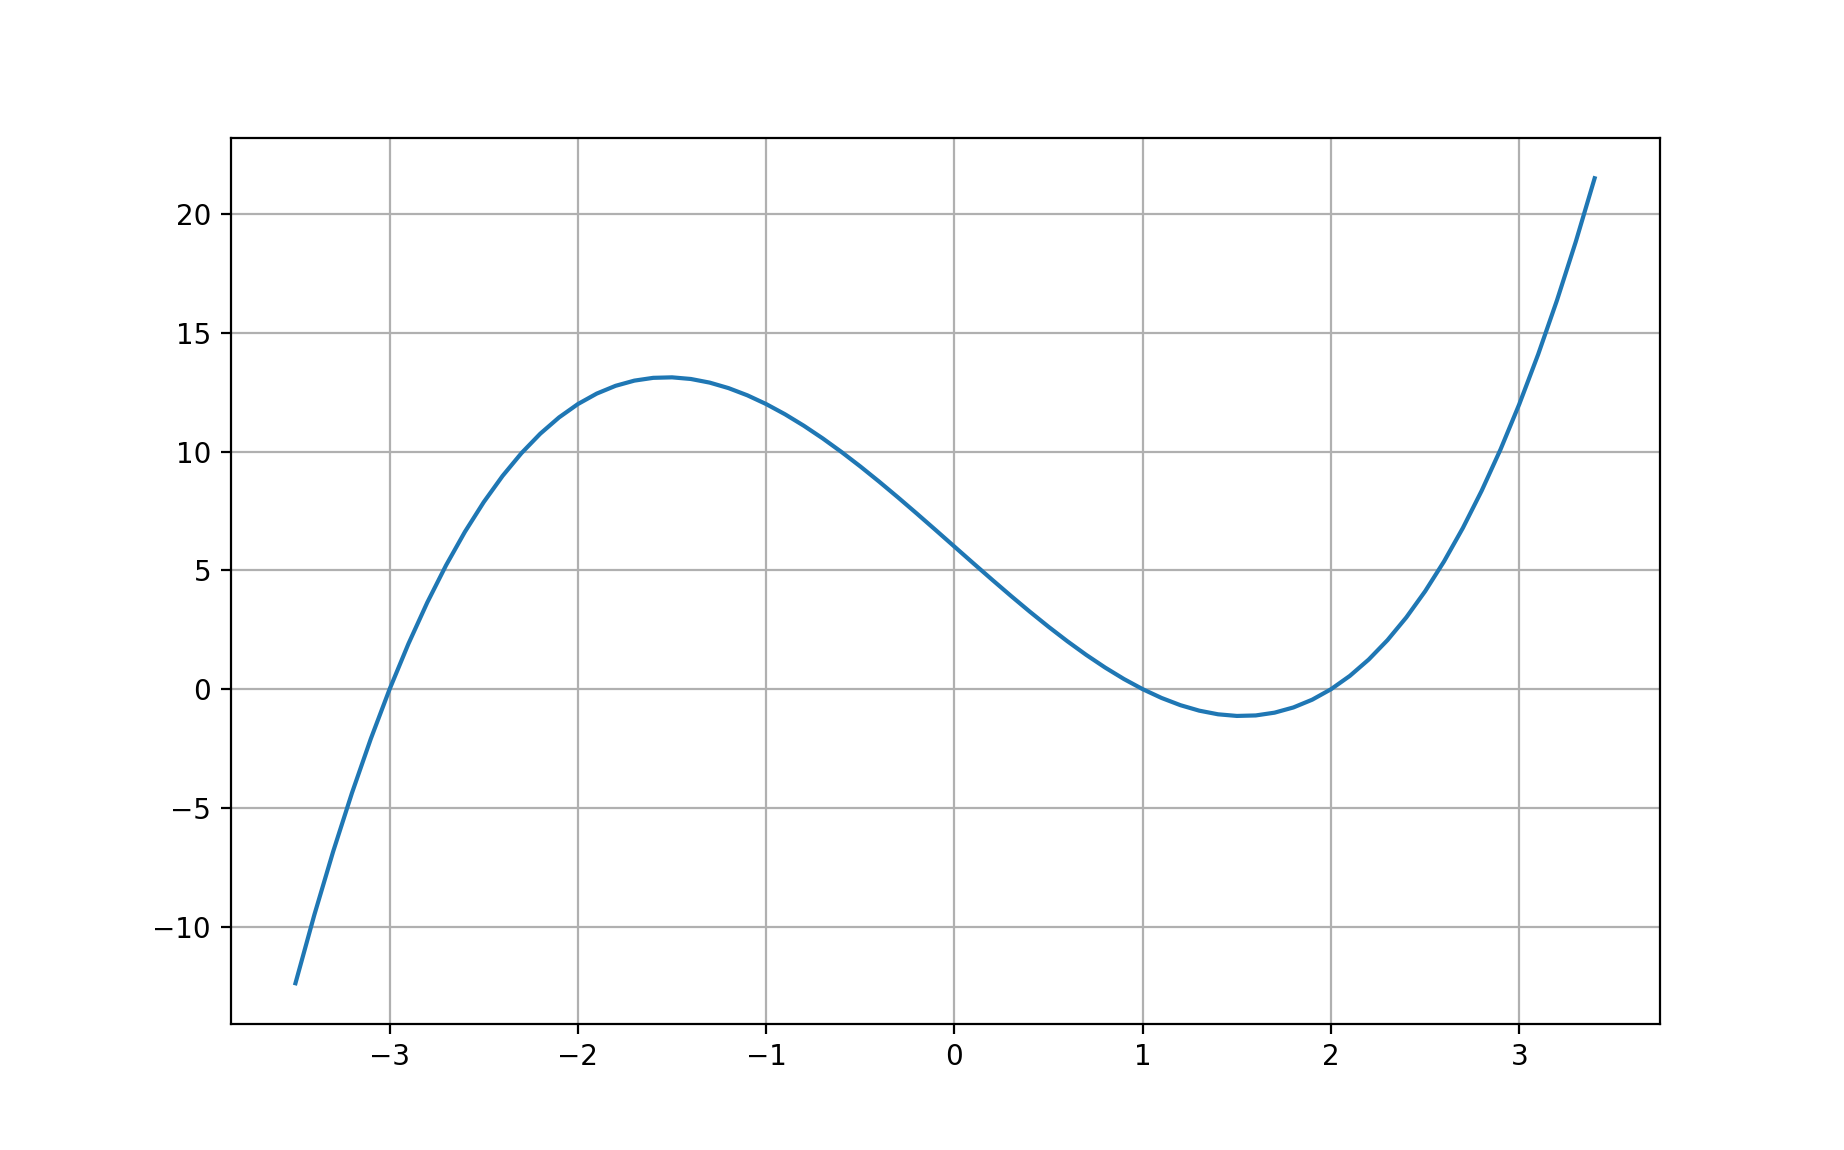
\includegraphics[width=\textwidth]{polyplot1.png}

If you received an error that the matplotlib was not found, use pip to install it:
\begin{Verbatim}[commandchars=\\\{\}]
$ \textbf{pip install matplotlib}
\end{Verbatim}
